\begin{figure}[H]
  \centering
  \resizebox{\textwidth}{!}{
  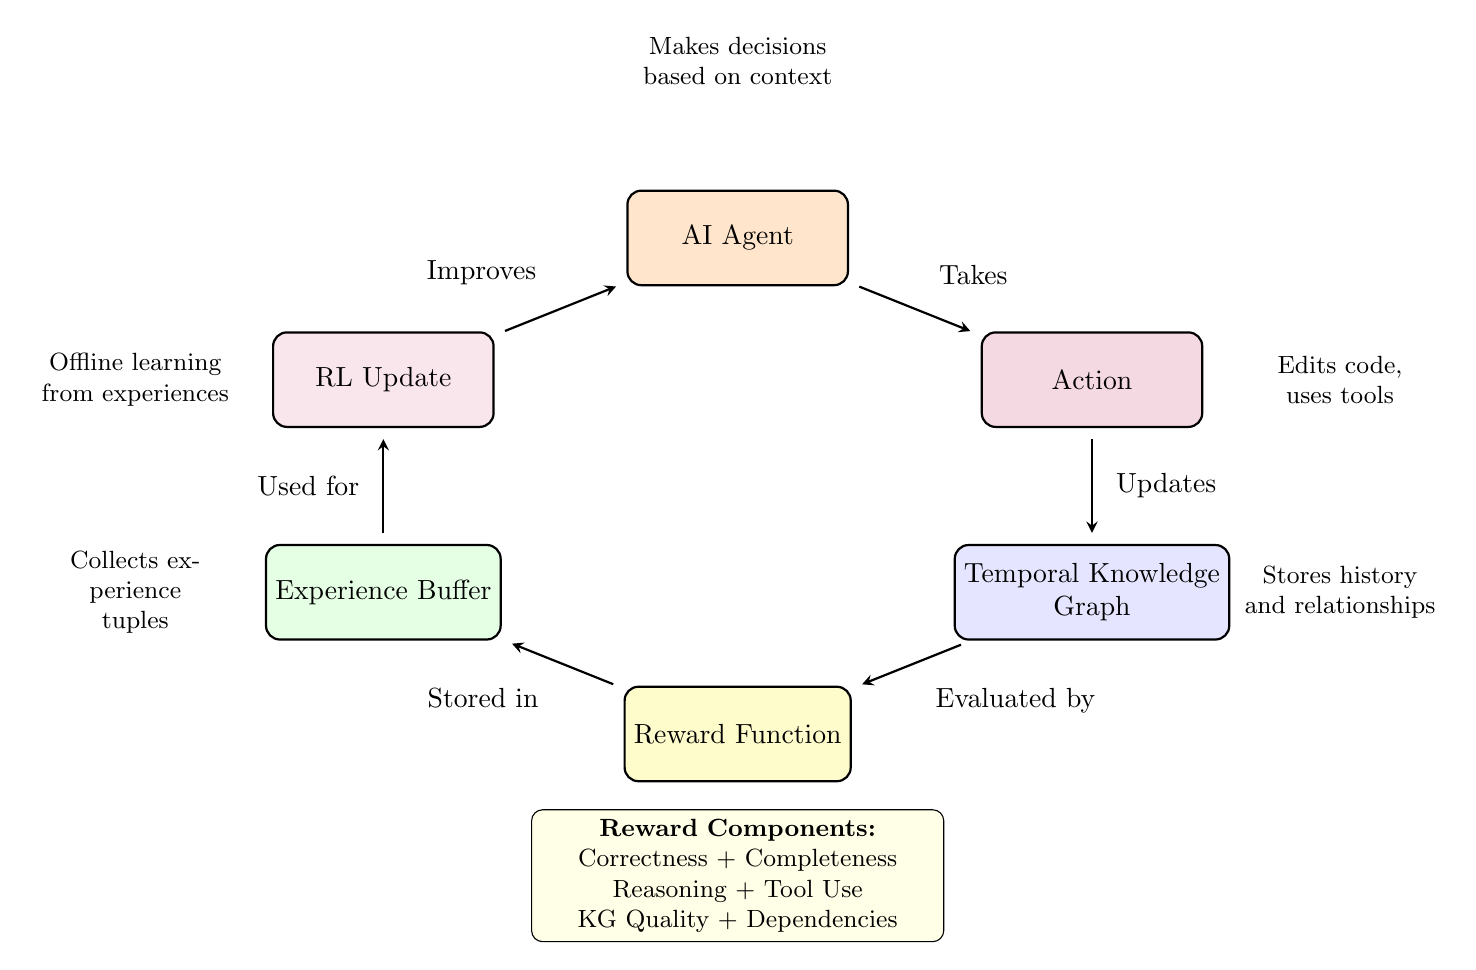
\begin{tikzpicture}[
    scale=0.9,
    box/.style={draw, minimum width=2.8cm, minimum height=1.2cm, align=center, rounded corners=5pt, thick},
    agent/.style={box, fill=orange!20},
    tkg/.style={box, fill=blue!10},
    action/.style={box, fill=purple!15},
    reward/.style={box, fill=yellow!20},
    buffer/.style={box, fill=green!10},
    arrow/.style={->, >=stealth, thick, shorten >=4pt, shorten <=4pt},
    dashedarrow/.style={->, >=stealth, thick, dashed, shorten >=4pt, shorten <=4pt}
  ]

  % Main components in a circular flow with increased spacing
  \node[agent] (agent) at (0,3.5) {AI Agent};
  \node[action] (action) at (5,1.5) {Action};
  \node[tkg] (tkg) at (5,-1.5) {Temporal Knowledge\\Graph};
  \node[reward] (reward) at (0,-3.5) {Reward Function};
  \node[buffer] (buffer) at (-5,-1.5) {Experience Buffer};
  \node[box, fill=purple!10] (rl) at (-5,1.5) {RL Update};

  % Simple circular flow with shorter labels and increased spacing
  \draw[arrow] (agent) -- node[above right, xshift=5pt, yshift=5pt] {Takes} (action);
  \draw[arrow] (action) -- node[right, xshift=5pt] {Updates} (tkg);
  \draw[arrow] (tkg) -- node[below right, xshift=5pt, yshift=-5pt] {Evaluated by} (reward);
  \draw[arrow] (reward) -- node[below left, xshift=-5pt, yshift=-5pt] {Stored in} (buffer);
  \draw[arrow] (buffer) -- node[left, xshift=-5pt] {Used for} (rl);
  \draw[arrow] (rl) -- node[above left, xshift=-5pt, yshift=5pt] {Improves} (agent);

  % Reward components with increased spacing
  \node[align=center, text width=5cm, font=\small, draw, fill=yellow!10, rounded corners] at (0,-5.5) {
    \textbf{Reward Components:}\\
    Correctness + Completeness\\
    Reasoning + Tool Use\\
    KG Quality + Dependencies
  };

  % Simple explanation of each component with increased spacing moved further out
  \node[align=center, text width=2.5cm, font=\small] at (0,6) {Makes decisions\\based on context};
  \node[align=center, text width=2.5cm, font=\small] at (8.5,1.5) {Edits code,\\uses tools};
  \node[align=center, text width=2.5cm, font=\small] at (8.5,-1.5) {Stores history\\and relationships};
  \node[align=center, text width=2.5cm, font=\small] at (-8.5,-1.5) {Collects experience\\tuples};
  \node[align=center, text width=2.5cm, font=\small] at (-8.5,1.5) {Offline learning\\from experiences};

  \end{tikzpicture}
  }
  \caption{Reinforcement Learning Flow in Arc: AI agents take actions that update the Temporal Knowledge Graph. These actions are evaluated by a multi-faceted reward function. The experiences are collected and used to improve agent policies through offline reinforcement learning.}
  \label{fig:rl_flow}
\end{figure}
